%%%%%%%%%%%%%%%%%%%%%%%%%%%%%%%%%%%%%%%%%
% a0poster Landscape Poster
% LaTeX Template
% Version 1.0 (22/06/13)
%
% The a0poster class was created by:
% Gerlinde Kettl and Matthias Weiser (tex@kettl.de)
%
% This template has been downloaded from:
% http://www.LaTeXTemplates.com
%
% License:
% CC BY-NC-SA 3.0 (http://creativecommons.org/licenses/by-nc-sa/3.0/)
%
%%%%%%%%%%%%%%%%%%%%%%%%%%%%%%%%%%%%%%%%%

%-------------------------------------------------------------------------------
%	PACKAGES AND OTHER DOCUMENT CONFIGURATIONS
%-------------------------------------------------------------------------------

\documentclass[a0, landscape]{a0poster}

\usepackage{multicol} % This is so we can have multiple columns of text side-by-side
\columnsep=100pt % This is the amount of white space between the columns in the poster
\columnseprule=3pt % This is the thickness of the black line between the columns in the poster

\usepackage[svgnames]{xcolor} % Specify colors by their 'svgnames', for a full list of all colors available see here: http://www.latextemplates.com/svgnames-colors

%\usepackage{times} % Use the times font
% \usepackage{palatino} % Uncomment to use the Palatino font
\usepackage{fontspec}
\setmainfont{Latin Modern Sans}

\usepackage{graphicx} % Required for including images
\graphicspath{{figures/}} % Location of the graphics files
\usepackage{booktabs} % Top and bottom rules for table
\usepackage[font=small,labelfont=bf]{caption} % Required for specifying captions to tables and figures
\usepackage{amsfonts, amsmath, amsthm, amssymb} % For math fonts, symbols and environments
\usepackage{wrapfig} % Allows wrapping text around tables and figures
\usepackage[export]{adjustbox}% http://ctan.org/pkg/adjustbox

\usepackage{listings}
\usepackage{color}
\usepackage{mathtools}

\newenvironment{Figure}
  {\par\medskip\noindent\minipage{\linewidth}}
  {\endminipage\par\medskip}

\DeclarePairedDelimiterX{\norm}[1]{\lVert}{\rVert}{#1}
\DeclareMathOperator{\Tr}{Tr}

\definecolor{dkgreen}{rgb}{0,0.6,0}
\definecolor{gray}{rgb}{0.5,0.5,0.5}
\definecolor{mauve}{rgb}{0.58,0,0.82}

\lstset{
  %frame=tb,
  language=Python,
  aboveskip=2mm,
  belowskip=0mm,
  showstringspaces=false,
  columns=flexible,
  basicstyle={\small\ttfamily},
  numbers=none,
  numberstyle=\tiny\color{gray},
  keywordstyle=\color{blue},
  commentstyle=\color{dkgreen},
  stringstyle=\color{mauve},
  breaklines=true,
  breakatwhitespace=true,
  tabsize=3,
  framexleftmargin=15pt
  }


\begin{document}

%----------------------------------------------------------------------------------------
%	POSTER HEADER
%----------------------------------------------------------------------------------------

% The header is divided into three boxes:
% The first is 55% wide and houses the title, subtitle, names and university/organization
% The second is 25% wide and houses contact information
% The third is 19% wide and houses a logo for your university/organization or a photo of you
% The widths of these boxes can be easily edited to accommodate your content as you see fit

\begin{minipage}[b]{0.88\linewidth}
\Large ~Poster W624\\

\veryHuge \color{NavyBlue} \textbf{DMRIprep: a Robust, Scalable Preprocessing Pipeline for Diffusion MRI} \color{Black}\\ % Title
%\Huge\textit{A really awesome subtitle}\\[1cm] % Subtitle
\huge \textbf{Adam Richie-Halford\textsuperscript{1}, Jason Yeatman\textsuperscript{2}, Ariel Rokem\textsuperscript{1}, Anisha Keshavan\textsuperscript{3}}\\ % Author(s)
\Large 1. University of Washington, 2. Stanford University, 3. Child Mind Institute \\ % University/organization
\Large Contact: \texttt{richford@uw.edu}
\end{minipage}
%
%\begin{minipage}[b]{0.25\linewidth}
%\color{DarkSlateGray}\Large \textbf{Contact Information:}\\
%Department Name\\ % Address
%University Name\\
%123 Broadway, State, Country\\\\
%Phone: +1 (000) 111 1111\\ % Phone number
%Email: \texttt{john@LaTeXTemplates.com}\\ % Email address
%\end{minipage}
%
\begin{minipage}[b]{0.19\linewidth}

\includegraphics[width=10cm]{UWlogo.png}
\end{minipage}

\vspace{0.5cm} % A bit of extra whitespace between the header and poster content

%----------------------------------------------------------------------------------------

\begin{multicols}{3} % This is how many columns your poster will be broken into, a poster with many figures may benefit from less columns whereas a text-heavy poster benefits from more

%----------------------------------------------------------------------------
%	Introduction
%----------------------------------------------------------------------------

\section*{Introduction}

\noindent Diffusion MRI (dMRI) is the only existing method to analyze human white matter \emph{in vivo}, but requires a pipeline of steps to preprocess the data, e.g.
\begin{itemize}
    \item eddy current correction,
    \item motion correction,
    \item adjustment of gradient direction.
\end{itemize}
Complexity and lack of standardization of these tasks can induce bias in subsequent interpretation of dMRI.

\\ \noindent {\Large Include figure from the ``pitfalls'' paper.} \\

\noindent In the field of fMRI, the FMRIprep software (Esteban et al.~2018) has successfully standardized fMRI preprocessing pipelines to reduce errors and increase reproducibility. Inspired by this success, DMRIprep applies the overarching philosophy of FMRIprep to dMRI analysis. It is designed to be
\begin{itemize}
    \item robust,
    \item reproducible,
    \item interrogable,
    \item scalable.
\end{itemize}

%----------------------------------------------------------------------------
%	Methods
%----------------------------------------------------------------------------

\section*{Methods}

\noindent DMRIprep is implemented as a nipype (Gorgolewski et al.~2011) workflow including
\begin{itemize}
    \item eddy current correction using FSL,
    \item coregistration to a T1W image with Freesurfer,
    \item the production of QC reports using
        \begin{itemize}
            \item FSL's EDDY QC framework (Bastiani et al.~2019),
            \item DIPY (Garyfallidis et al.~2014),
        \end{itemize}
    \item a custom interactive report website.
\end{itemize}

\begin{Figure}
    \centering
    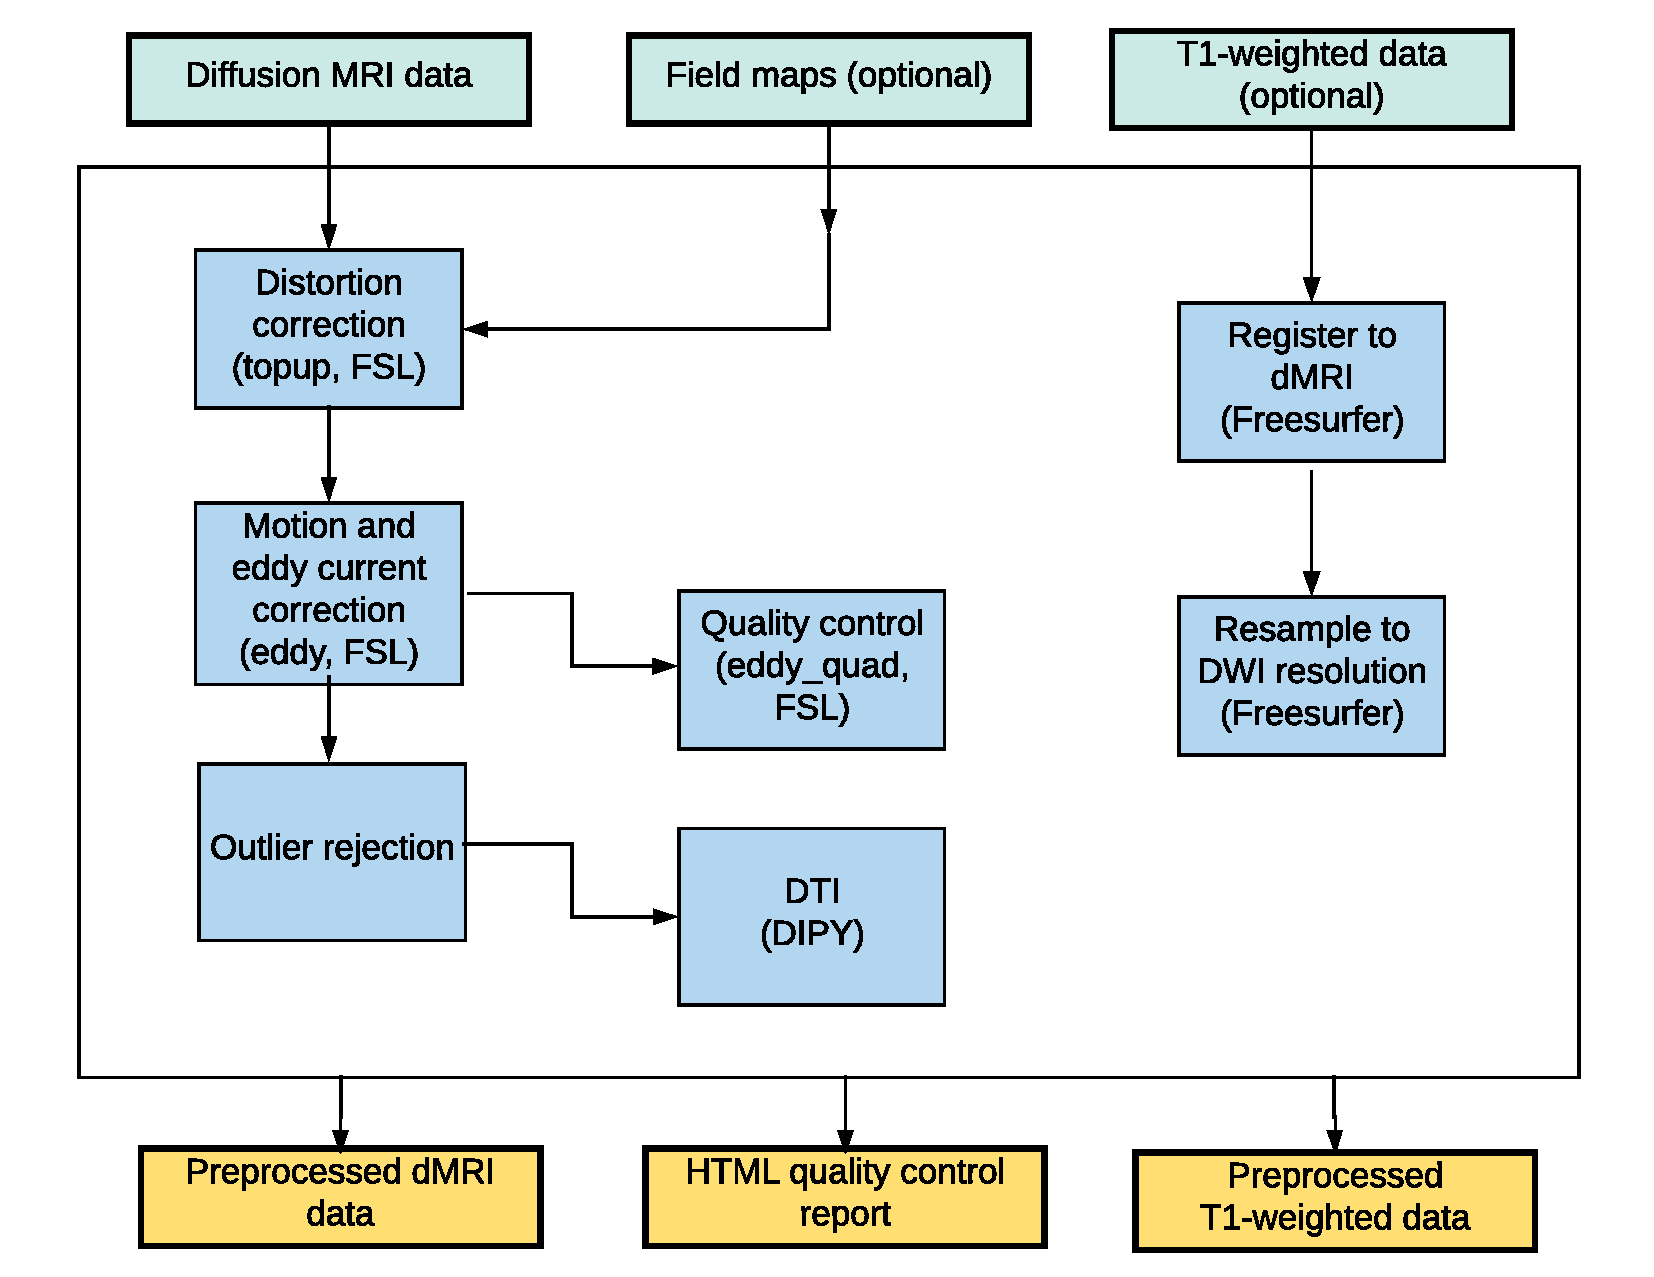
\includegraphics[width=0.8\linewidth]{dmriprep_workflow.pdf}
    \captionof{figure}{The DMRIprep workflow: given input dMRI data and (optional) EPI field maps, FSL's topup and eddy programs correct for distortions, subject movement, and eddy currents. DMRIprep removes volumes that exceed a user-defined threshold for the number of outlier slices. Eddy Quad operates on the output of eddy to generate QC reports, which are organized into an interactive report webpage (see Figure 2). Dipy computes the diffusion tensor images of the corrected dMRI data. Separately, the input structural images are registered to the dMRI data and resampled to DWI resolution using Freesurfer. The preprocessed T1w and dMRI data are organized in BIDS format for further dMRI analysis.}
\end{Figure}

\vfill
\columnbreak

\noindent All DMRIprep dependencies are packaged into a Docker image with three command line tools:
\begin{itemize}
    \item \texttt{dmriprep}: a BIDS-App compliant tool that runs the primary workflow,
    \item \texttt{dmriprep-data}: a tool to download data from public datasets and transform the files to BIDS-format,
    \item \texttt{dmriprep-upload}: a tool to upload DMRIprep results to an Amazon Web Services (AWS) S3 bucket.
\end{itemize}

\color{Navy}

%----------------------------------------------------------------------------
%	RESULTS
%----------------------------------------------------------------------------

\section*{Results}

\noindent We tested DMRIprep by analyzing the Healthy Brain Network (HBN; Alexander et al.~2017) dataset.
\begin{itemize}
    \item 60 subjects from three different sites (``Site-SI'', ``Site-RU'', ``Site-CBIC'')
    \item BIDS compliant (mostly)
    \item DMRIprep was able to accommodate slight irregularities in each site's file structure and format.
    \item Visually inspected QC results using DMRIprep-viewer (\texttt{http://nipy.org/dmriprep}).
\end{itemize}

\begin{Figure}
    \centering
    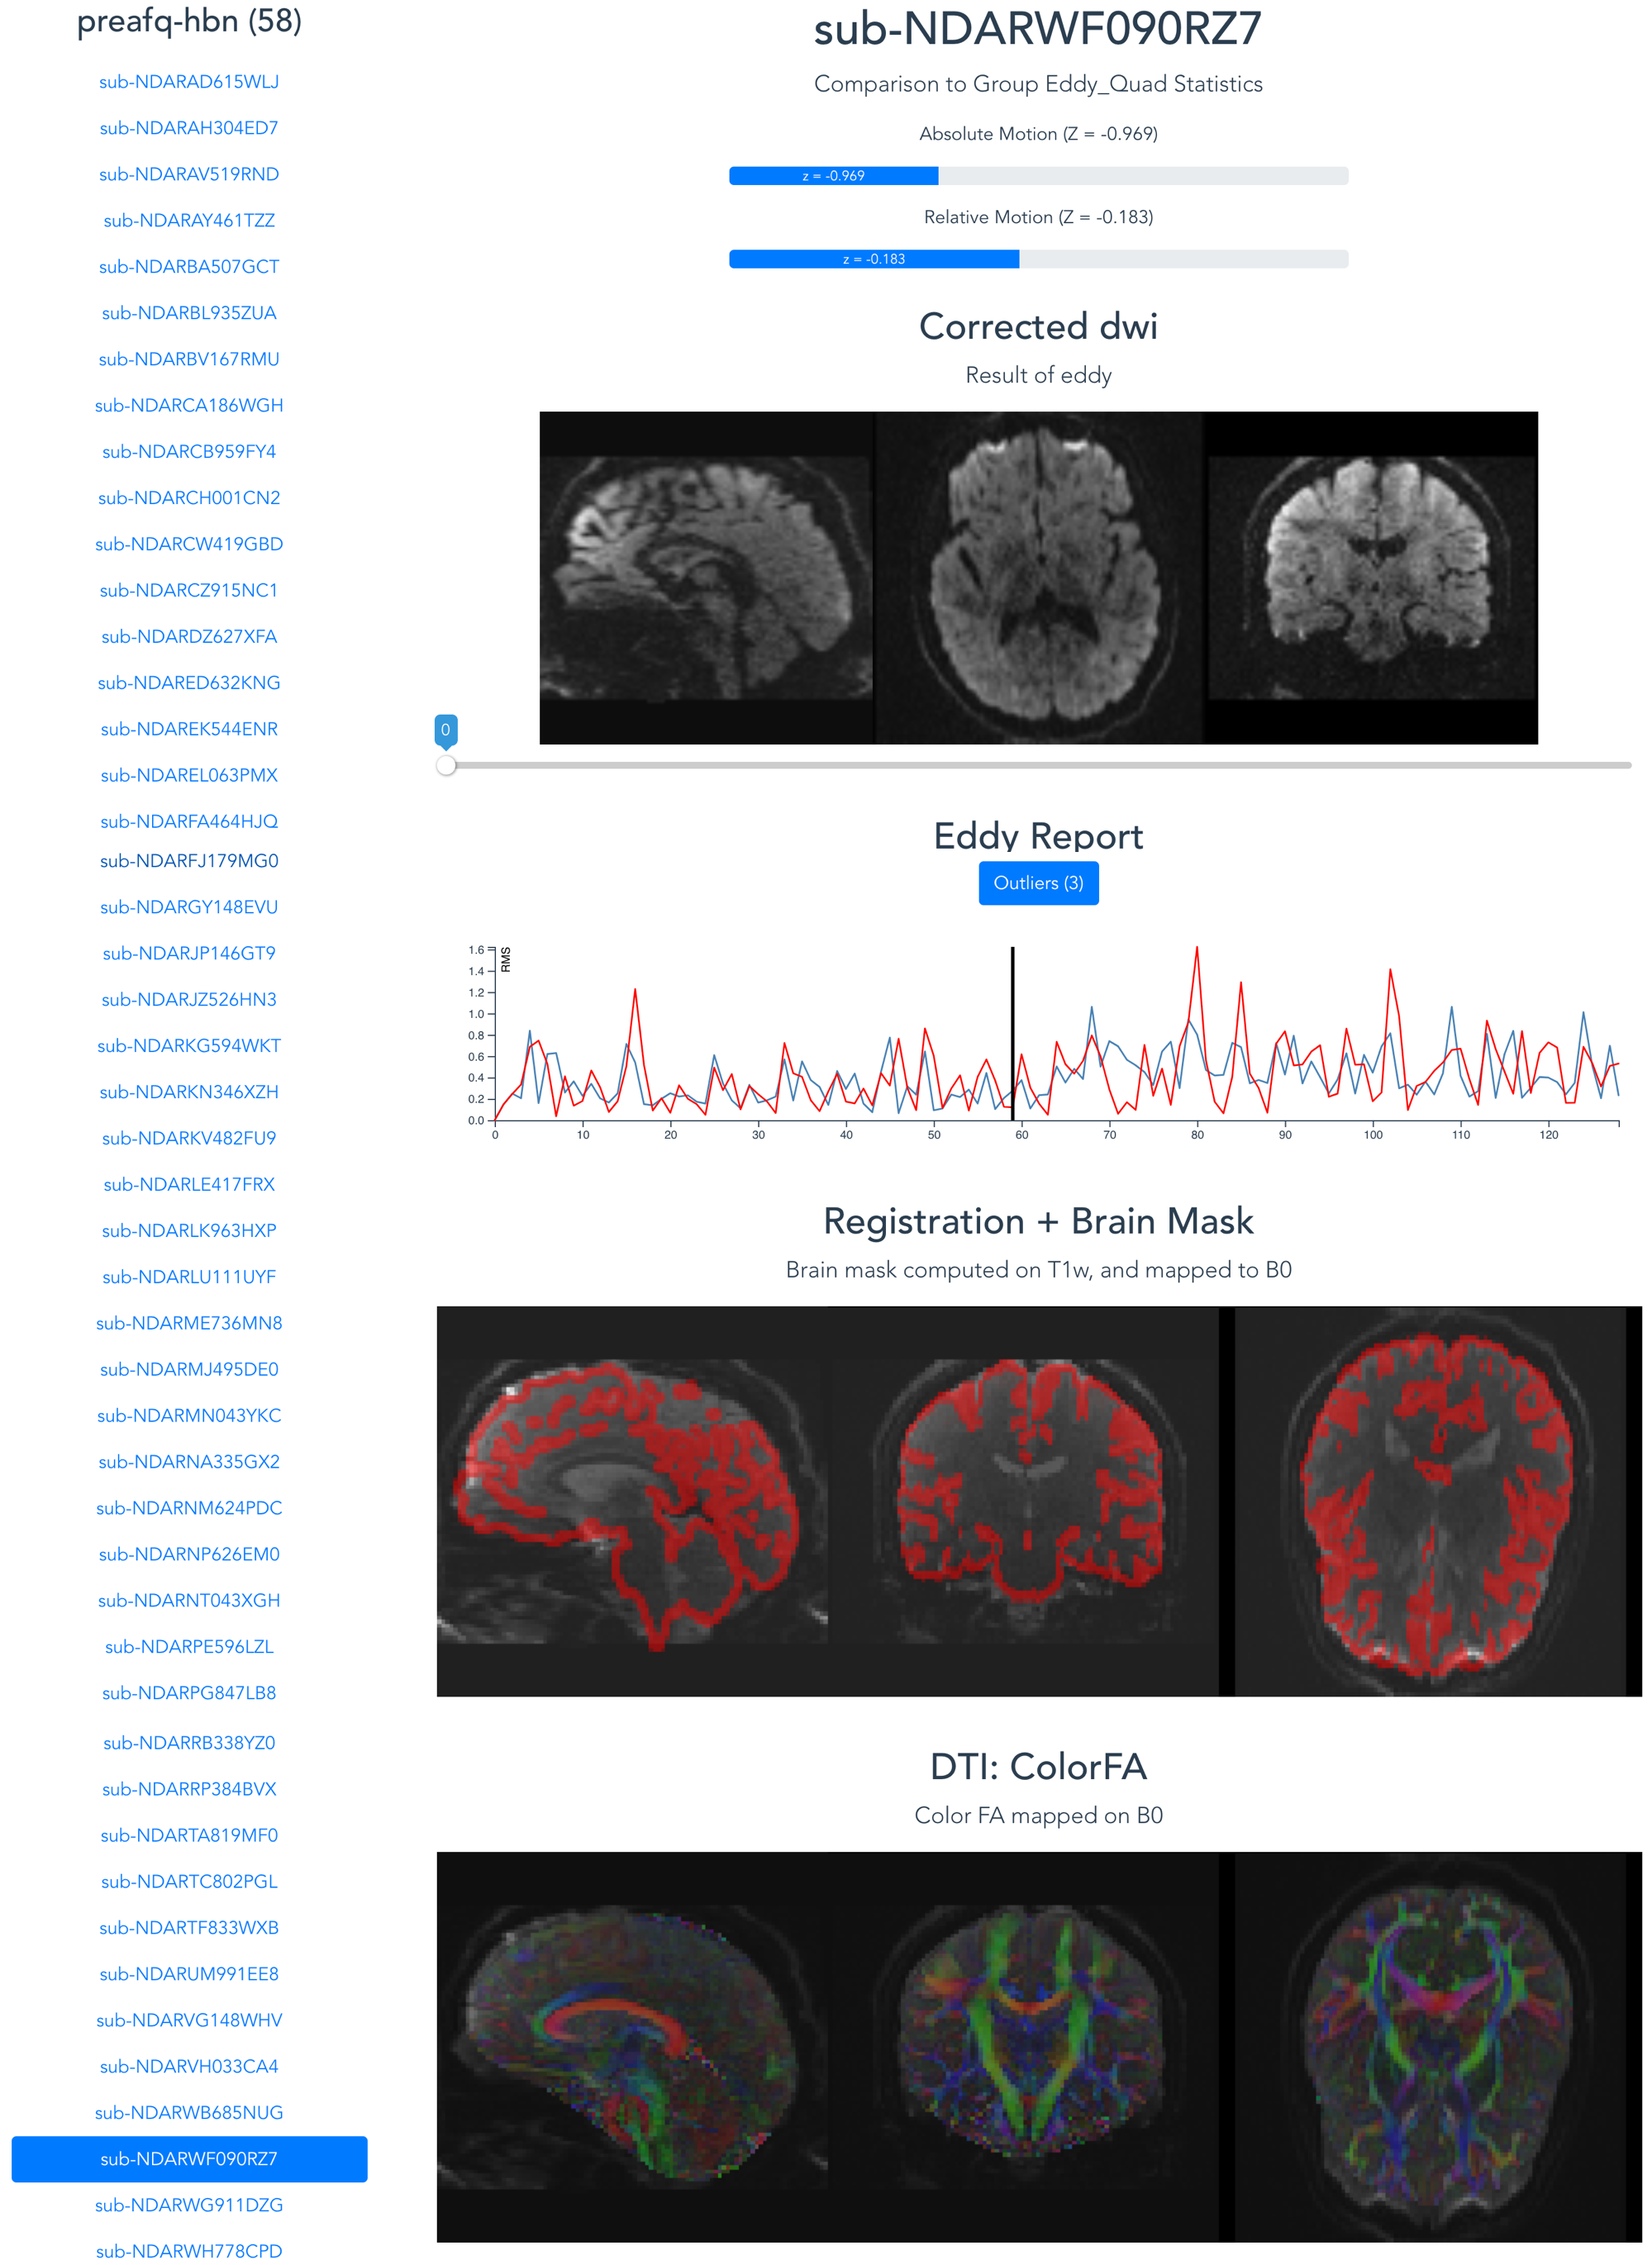
\includegraphics[width=0.9\linewidth]{qc_report.png}
    \captionof{figure}{\color{Navy} An example DMRIprep QC report, generated with DMRIprep-viewer. From top to bottom, it displays: (1) group comparisons for relative and absolute motion; (2) a view of the eddy current-corrected DWI volumes; (3) a report of the outlier volumes and slices; (4) a view of the registration mask, mapped onto the B0 DWI images; and (5) a DTI map showing fractional anisotropy mapped onto the B0 image.}
\end{Figure}

\vfill
\columnbreak

\begin{minipage}[b]{0.45\linewidth}
\begin{Figure}
    \centering
    
\includegraphics[width=0.5\linewidth]{dmriprep_qc_dynamic_qr.png}\\
    \color{Navy} \textbf{Interactive QC report}
\end{Figure}
\end{minipage}
\begin{minipage}[b]{0.45\linewidth}
\begin{Figure}
    \centering
    
\includegraphics[width=0.5\linewidth]{dmriprep_github_dynamic_qr.png}\\
    \color{Navy} \textbf{GitHub repository}
\end{Figure}
\end{minipage}

\begin{itemize}
    \item Preprocessing failed gracefully on two of the 60 subjects due to data acquisition errors (the b-values and b-vectors did not match the total number of volumes in the image).
    \item Running 60 subjects on Google Cloud Platform (GCP) using Kubernetes cost 51~USD in total, approximately 0.85~USD per subject (using an n1-highmem-4 machine with 26GB RAM and 4 vCPUs.
\end{itemize}

\color{SaddleBrown} % SaddleBrown color for the conclusions to make them stand out

\section*{Conclusions}

\begin{itemize}
    \item DMRIprep implements
    \begin{itemize}
        \item a nipype pipeline for preprocessing of dMRI data,
        \item web-based visualizations for quality control of results,
        \item a BIDS-App compliant command-line interface to download, preprocess, and upload large dMRI datasets.
    \end{itemize}

    \item Robust, scalable preprocessing pipeline for many different experimental settings.
    \item Improves consistency and reproducibility of analysis procedures and methods reporting.
    \item Packaged as open-source software: \texttt{https://github.com/nipy/dmriprep}
\end{itemize}

\color{DarkSlateGray} % Set the color back to DarkSlateGray for the rest of the content

%----------------------------------------------------------------------------
%   REFERENCES
%----------------------------------------------------------------------------

\nocite{*} % Print all references regardless of whether they were cited in the poster or not
\bibliographystyle{plain} % Plain referencing style
\footnotesize \bibliography{poster} % Use the example bibliography file sample.bib

%----------------------------------------------------------------------------
%	ACKNOWLEDGEMENTS
%----------------------------------------------------------------------------
\subsection*{Acknowledgements} \footnotesize


\includegraphics[height=2.6cm]{SloanLogo.png}

\includegraphics[height=2.6cm]{MooreFdn.png}

\includegraphics[height=2.6cm]{eSciencelogo.png}
%----------------------------------------------------------------------------

\end{multicols}
\end{document}
